\chapter{Análise dos Resultados}
\label{cap:04}
Neste capítulo, são apresentados e discutidos os resultados obtidos na aplicação dos métodos de segmentação de imagens propostos neste trabalho, com ênfase nas imagens de média e baixa resolução. Utilizando o modelo Segment Anything (SAM), avaliou-se a eficácia do método utilizado, que utilize inteligencia artificial para aprimorar a precisão da segmentação.

Para uma análise quantitativa robusta, foram adotadas as métricas Mean Squared Error (MSE) e Normalized Cross-Correlation (NCC), além de um método específico criado para complementar a avaliação dos segmentos. Estes indicadores foram aplicados para avaliar a qualidade das segmentações produzidas, comparando-as com padrões de segmentação existentes. Este capítulo tem, portanto, como objetivo apresentar as análises qualitativas e quantitativas dos resultados, destacando os avanços e as limitações do método proposto em relação aos métodos tradicionais.

\section{Agilidade e Eficiência}
Nessa seção será abordado o fator velocidade para o processo ser finalizado, ou seja, independente dos resultados qual a margem de tempo destinada apenas a realização da segmentação das imagens, lembrando que isso seria apenas um fragmento de todo o desenvolvimento da ferramenta.

Como o esperado, foi identificado nos computadores usados para executar o código uma quantidade de tempo razoável até sua finalização,apesar disso, entre eles houveram minímas diferenças de tempo de execução, mesmo com abruptas diferenças de processamento, em seguida será mostrado as propriedades de cada um deles, para uma melhor comparação da média dos resultados obtidos em termos de desempenho, como mostra a \ref{tab:comparacao_desempenho}.

\begin{table}[h!]
	\centering
	\begin{tabular}{|p{4cm}|p{5cm}|p{5cm}|}
	\hline
	\textbf{Propriedade}         & \textbf{Computador}                & \textbf{Notebook}                     \\ \hline
	\textbf{Processador}          & AMD Ryzen 5 1400 Quad-Core        & Intel Core i5-1235U                   \\ \hline
	\textbf{Número de Threads}    & 8                                 & 12                                    \\ \hline
	\textbf{Frequência Base}      & 99.8 MHz                          & 99.8 MHz                              \\ \hline
	\textbf{Frequência Máxima}    & 3192.4 MHz                        & 3790.7 MHz                            \\ \hline
	\textbf{Memória RAM}          & 16 GB DDR4                        & 8 GB DDR4                             \\ \hline
	\textbf{Frequência da Memória}& Não especificada                  & 1596.1 MHz                            \\ \hline
	\textbf{\textit{Chipset}}     & AMD B350                          & Intel Alder Lake rev. 04              \\ \hline
	\textbf{Placa Mãe}            & Asus Prime A320M-K/BR             & Modelo LNVNB161216                    \\ \hline
	\textbf{\footnote{VRAM}}      & 4 GB NVIDIA 1050 TI               & Intel UHD Graphics                    \\ \hline
	\end{tabular}
	\caption{Comparação de Desempenho entre Computador e Notebook}
	\label{tab:comparacao_desempenho}
\end{table}

Com a tabela é possível notar que apesar da comparação semelhante quando nos referimos ao processamento das maquinas, é extremamente necessário levar em consideração o uso da placa gráfica para o processamento com o suporte do CUDA, que nada mais é do que um sistema criado pela NVIDIA a fim de utilizar as placas gráficas como potencializadores para integração de inteligências artificiais, contudo, os resultados em termos de velocidade de execução foram muito próximos como é possível notar no gráfico \ref{fig:grafico_desempenho}

\FloatBarrier
\begin{figure}[ht]
    \caption{Análise de desempenho}
    \centering
    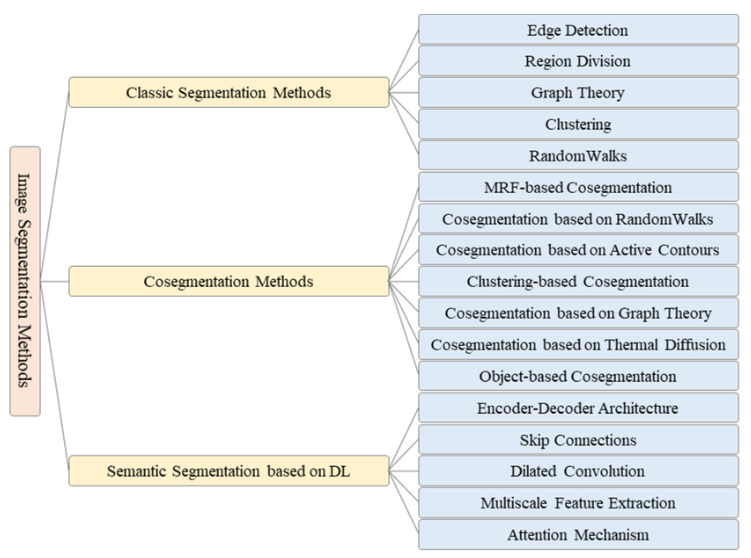
\includegraphics[scale=0.5]{imagens/metodos_segmentacao.png}
    \label{fig:grafico_desempenho}
\end{figure}
\FloatBarrier


\section{Resultados/Impactos}

Resultados.

\section{Cronograma do Trabalho}

Segue abaixo o cronograma de trabalho das atividades realizadas até a Avaliação Final de TCC.

\begin{enumerate}
	\item Elaboração da Introdução
	\item Elaboração da Revisão da Literatura
	\item Elaboração da Metodologia
	\item Estudo sobre a \textit{Unity} e Iluminação
	\item Desenvolvimento da ferramenta
    \item Alteração do escopo em decorrência das dificuldades técnicas 
    \item Geração das imagens para análise
    \item Análise e elaboração das métricas
    \item Desenvolvimento dos capítulos
    \item Revisão e Conclusão
\end{enumerate}

\FloatBarrier
\begin{figure*}[!htbp]
	\centering
	\includegraphics[scale=0.8]{imagens/Cronograma.png}
\end{figure*}
\FloatBarrier


